\documentclass[tikz,border=10pt]{standalone}
\usepackage{amsmath}
\usetikzlibrary{arrows.meta, positioning, calc, decorations.pathreplacing}
\definecolor{c1}{HTML}{000000}
\definecolor{c2}{HTML}{233D4D}
\definecolor{c3}{HTML}{FE7F2D}
\definecolor{c4}{HTML}{EAECF0}
\definecolor{axiscolor}{HTML}{333333}
\definecolor{labelcolor}{HTML}{5F6B75}
\begin{document}
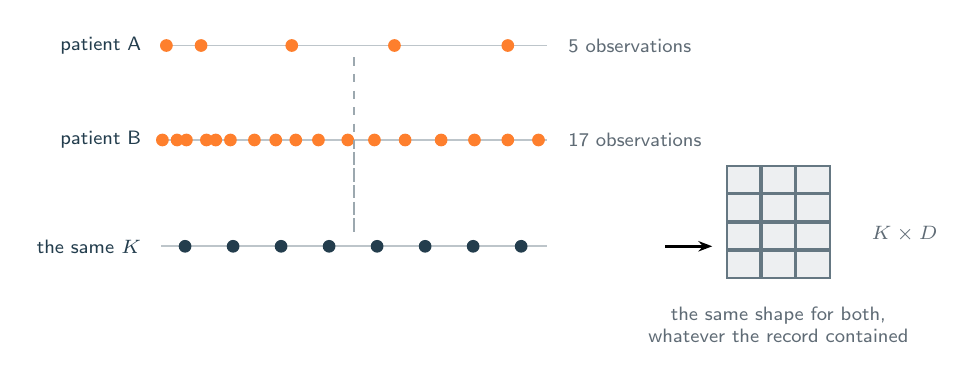
\begin{tikzpicture}[
    every node/.style={font=\sffamily},
    lab/.style={font=\sffamily\scriptsize, text=labelcolor},
    tag/.style={font=\sffamily\scriptsize, text=c2},
    arr/.style={-{Stealth[length=5pt]}, line width=1.0pt, color=c1},
    cell/.style={rectangle, draw=c2!70, fill=c2!8, line width=0.7pt,
                 minimum width=0.42cm, minimum height=0.34cm},
]
\def\X#1{1.55 + #1*0.001700}

% patient A: five observations
\node[tag, anchor=east] at (1.42, 4.75) {patient A};
\draw[c2!30, line width=0.7pt] (1.55, 4.75) -- (6.45, 4.75);
\foreach \m in {40, 300, 980, 1750, 2600}{
    \fill[c3] ({\X{\m}}, 4.75) circle (2.3pt);
}
\node[lab, anchor=west] at (6.60, 4.75) {5 observations};

% patient B: seventeen observations
\node[tag, anchor=east] at (1.42, 3.55) {patient B};
\draw[c2!30, line width=0.7pt] (1.55, 3.55) -- (6.45, 3.55);
\foreach \m in {10,120,190,340,410,520,700,860,1010,1180,1400,1600,1830,2100,2350,2600,2830}{
    \fill[c3] ({\X{\m}}, 3.55) circle (2.3pt);
}
\node[lab, anchor=west] at (6.60, 3.55) {17 observations};

% the shared reference points
\node[tag, anchor=east] at (1.42, 2.20) {the same $K$};
\draw[c2!30, line width=0.7pt] (1.55, 2.20) -- (6.45, 2.20);
\foreach \k in {0,...,7}{
    \pgfmathsetmacro\m{180 + \k*360}
    \fill[c2] ({\X{\m}}, 2.20) circle (2.3pt);
}
\draw[c2!45, line width=0.7pt, dashed] (4.00, 4.60) -- (4.00, 2.35);
\draw[c2!45, line width=0.7pt, dashed] (4.00, 3.40) -- (4.00, 2.35);

\draw[arr] (7.95, 2.20) -- (8.55, 2.20);

% the output block
\foreach \r in {0,...,3}{
    \foreach \c in {0,...,2}{
        \node[cell] at ({8.95 + \c*0.44}, {3.05 - \r*0.36}) {};
    }
}
\node[lab, anchor=west] at (10.45, 2.35) {$K \times D$};
\node[lab, anchor=north, align=center] at (9.39, 1.55)
    {the same shape for both,\\ whatever the record contained};
\end{tikzpicture}
\end{document}
